\subsection{Sensorik}
\subsubsection{Gyroskop}
Funktionsweise
Tiefpassfilter
Bias-Korrektur
HBW \& LBW Fusion
Wertebereiche, wie alte Präsentation
Integration
Eigenschaften (schnell, aber Drift durch Integration)
\subsubsection{Beschleunigungssensor}
Funktionsweise
für Roll und Pitch
Tiefpassfilter
Umrechnung auf m/s$^2$
Berechnung von Roll und Pitch direkt aus Werten
Problem: ungenügendes Yaw
\subsubsection{Magnetometer}
Funktionsweise

\begin{figure}
   \centering
   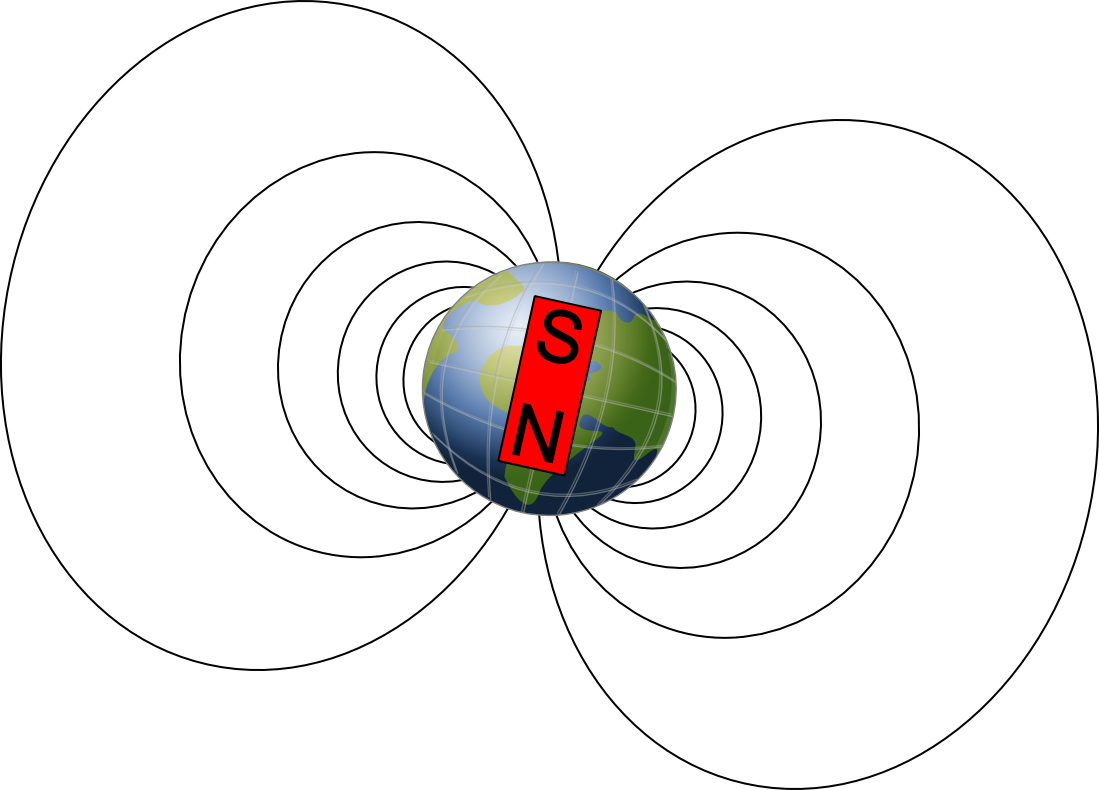
\includegraphics[width=0.3\textwidth]{earth-magnetic-field}
   \caption[Test]{Test Test}
   \label{fig:headtracking_test}
\end{figure}

Tiefpassfilter
Magnetometer-Bias-Korrektur (durch Min/Max-Werte), Normierung auf [-1,1]
Magnetometer-Kreisplots vor/nach Kalibrierung, Magnetometer-Fehler in Kreisplots
Transformation auf XY Ebene (Algorithmus Ralf)
\subsubsection{Kamera}